\documentclass[tikz,border=5pt]{standalone}
\usepackage{tikz}
\usepackage{pgfplots}
\usepgfplotslibrary{groupplots}
\pgfplotsset{compat=1.18}
% sha256: e61a48bcd0d6abc4407fab150d65aaa7438314b1cd3cc23862409c3638582005
\definecolor{p06color0}{HTML}{0072B2}
\definecolor{p06color1}{HTML}{009E73}
\definecolor{p06color2}{HTML}{D55E00}
\begin{document}
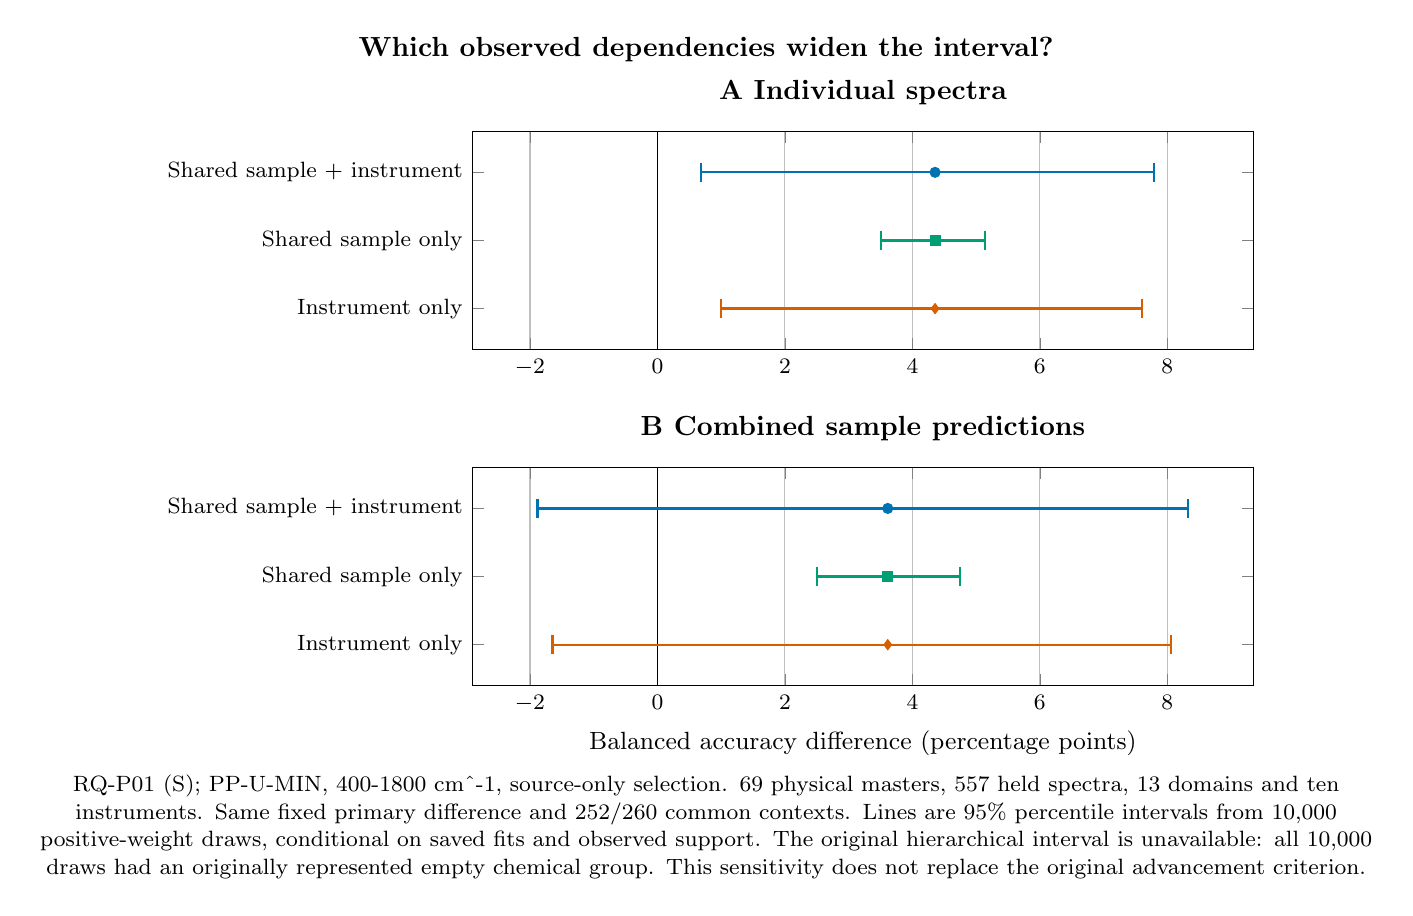
\begin{tikzpicture}
\begin{groupplot}[group style={group size=1 by 2, vertical sep=1.5cm},
width=11.5cm,
height=4.35cm,
xmin=-2.90266642679674, xmax=9.35007957499599,
tick label style={font=\fontsize{8}{10}\selectfont, color=black},
yticklabel style={font=\fontsize{8}{10}\selectfont, color=black},
title style={font=\bfseries\fontsize{10}{12}\selectfont, color=black},
xlabel style={font=\fontsize{9}{11}\selectfont, color=black},
xmajorgrids=true,
ymajorgrids=false]
\nextgroupplot[title={A Individual spectra}, ytick={1,2,3}, yticklabels={Instrument only,Shared sample only,Shared sample + instrument}, ymin=0.4, ymax=3.6]
\addplot[forget plot, black, thin] coordinates {(0,0.4) (0,3.6)};
\addplot[forget plot, color=p06color2, thick] coordinates {(0.999322571300504,1) (7.60532821131661,1)};
\addplot[forget plot, color=p06color2, thick] coordinates {(0.999322571300504,0.86) (0.999322571300504,1.14)};
\addplot[forget plot, color=p06color2, thick] coordinates {(7.60532821131661,0.86) (7.60532821131661,1.14)};
\addplot[only marks, mark=diamond*, mark size=1.8pt, color=p06color2] coordinates {(4.35573093248532,1)};
\addplot[forget plot, color=p06color1, thick] coordinates {(3.51304177268609,2) (5.139046495494,2)};
\addplot[forget plot, color=p06color1, thick] coordinates {(3.51304177268609,1.86) (3.51304177268609,2.14)};
\addplot[forget plot, color=p06color1, thick] coordinates {(5.139046495494,1.86) (5.139046495494,2.14)};
\addplot[only marks, mark=square*, mark size=1.8pt, color=p06color1] coordinates {(4.35573093248532,2)};
\addplot[forget plot, color=p06color0, thick] coordinates {(0.68373247447679,3) (7.79477318696698,3)};
\addplot[forget plot, color=p06color0, thick] coordinates {(0.68373247447679,2.86) (0.68373247447679,3.14)};
\addplot[forget plot, color=p06color0, thick] coordinates {(7.79477318696698,2.86) (7.79477318696698,3.14)};
\addplot[only marks, mark=*, mark size=1.8pt, color=p06color0] coordinates {(4.35573093248532,3)};
\nextgroupplot[title={B Combined sample predictions}, xlabel={Balanced accuracy difference (percentage points)}, ytick={1,2,3}, yticklabels={Instrument only,Shared sample only,Shared sample + instrument}, ymin=0.4, ymax=3.6]
\addplot[forget plot, black, thin] coordinates {(0,0.4) (0,3.6)};
\addplot[forget plot, color=p06color2, thick] coordinates {(-1.64738711056304,1) (8.05189764885036,1)};
\addplot[forget plot, color=p06color2, thick] coordinates {(-1.64738711056304,0.86) (-1.64738711056304,1.14)};
\addplot[forget plot, color=p06color2, thick] coordinates {(8.05189764885036,0.86) (8.05189764885036,1.14)};
\addplot[only marks, mark=diamond*, mark size=1.8pt, color=p06color2] coordinates {(3.61373519268256,1)};
\addplot[forget plot, color=p06color1, thick] coordinates {(2.50473837224657,2) (4.75210372098555,2)};
\addplot[forget plot, color=p06color1, thick] coordinates {(2.50473837224657,1.86) (2.50473837224657,2.14)};
\addplot[forget plot, color=p06color1, thick] coordinates {(4.75210372098555,1.86) (4.75210372098555,2.14)};
\addplot[only marks, mark=square*, mark size=1.8pt, color=p06color1] coordinates {(3.61373519268256,2)};
\addplot[forget plot, color=p06color0, thick] coordinates {(-1.88160425998068,3) (8.32901740817993,3)};
\addplot[forget plot, color=p06color0, thick] coordinates {(-1.88160425998068,2.86) (-1.88160425998068,3.14)};
\addplot[forget plot, color=p06color0, thick] coordinates {(8.32901740817993,2.86) (8.32901740817993,3.14)};
\addplot[only marks, mark=*, mark size=1.8pt, color=p06color0] coordinates {(3.61373519268256,3)};
\end{groupplot}
\node[anchor=south, font=\bfseries\fontsize{10}{12}\selectfont] at (current bounding box.north) {Which observed dependencies widen the interval?};
\node[anchor=north, text width=17cm, align=center, font=\fontsize{8}{10}\selectfont] at (current bounding box.south) {RQ-P01 (S); PP-U-MIN, 400-1800 cm\textasciicircum{}-1, source-only selection. 69 physical masters, 557 held spectra, 13 domains and ten instruments. Same fixed primary difference and 252/260 common contexts. Lines are 95\% percentile intervals from 10,000 positive-weight draws, conditional on saved fits and observed support. The original hierarchical interval is unavailable: all 10,000 draws had an originally represented empty chemical group. This sensitivity does not replace the original advancement criterion.};
\end{tikzpicture}
\end{document}
